\documentclass[conference]{IEEEtran}
\usepackage[T1]{fontenc} % Times under XeTeX (tectonic) as well as pdfLaTeX
\usepackage{amsmath,amssymb,array,booktabs,graphicx,cite,url,microtype}
% generated by report/make_tables.py - do not edit
\newcommand{\NPresentations}{\mbox{22}}
\newcommand{\NRegistrations}{\mbox{32,593}}
\newcommand{\NAssessRecords}{\mbox{173,912}}
\newcommand{\PassRate}{\mbox{94\%}}
\newcommand{\SubmitRate}{\mbox{80\%}}
\newcommand{\TestStudents}{\mbox{3,064}}
\newcommand{\TestRows}{\mbox{14,976}}
\newcommand{\HoldRows}{\mbox{24,122}}
\newcommand{\HoldStudents}{\mbox{4,526}}
\newcommand{\WeekMapDDD}{\mbox{0.1\%}}
\newcommand{\WeekMapFFF}{\mbox{42\%}}
\newcommand{\InterestActivityR}{\mbox{0.03}}
\newcommand{\InterestSplitHalf}{\mbox{0.49}}
\newcommand{\FixedS}{\mbox{120}}
\newcommand{\AucTopicOne}{\mbox{0.848}}
\newcommand{\AucNone}{\mbox{0.900}}
\newcommand{\AucLearned}{\mbox{0.902}}
\newcommand{\AucGain}{\mbox{$+$0.0018}}
\newcommand{\AucGainLo}{\mbox{$+$0.0002}}
\newcommand{\AucGainHi}{\mbox{$+$0.0037}}
\newcommand{\HoldGain}{\mbox{$-$0.0004}}
\newcommand{\HoldGainLo}{\mbox{$-$0.0011}}
\newcommand{\HoldGainHi}{\mbox{$+$0.0002}}
\newcommand{\HoldDasGap}{\mbox{0.011}}
\newcommand{\RankRandom}{\mbox{0.739}}
\newcommand{\RankPop}{\mbox{0.946}}
\newcommand{\RankMastery}{\mbox{0.653}}
\newcommand{\RankThree}{\mbox{0.828}}
\newcommand{\RankFive}{\mbox{0.840}}
\newcommand{\RankThreeB}{\mbox{0.553}}
\newcommand{\RankFiveB}{\mbox{0.805}}
\newcommand{\SensSeventy}{\mbox{$+$0.013}}
\newcommand{\SensNonsub}{\mbox{$+$0.020}}
\newcommand{\SensData}{\mbox{$-$0.091}}
\newcommand{\HoldPop}{\mbox{0.893}}
\newcommand{\HoldForget}{\mbox{$+$0.009}}
\newcommand{\HoldForgetB}{\mbox{$-$0.004}}
\newcommand{\HoldInterest}{\mbox{$+$0.014}}
\newcommand{\HoldPopGap}{\mbox{0.165}}
\newcommand{\PostForget}{\mbox{0.000}}
\newcommand{\ExamGap}{\mbox{$-$0.088}}
\newcommand{\DeltaTwo}{\mbox{188}}
\newcommand{\DeltaFive}{\mbox{83}}
\newcommand{\ResetFive}{\mbox{20\%}}
\newcommand{\ResetThree}{\mbox{34\%}}
\newcommand{\ResetSix}{\mbox{90\%}}
\newcommand{\NavLow}{\mbox{32\%}}
\newcommand{\NavHigh}{\mbox{61\%}}
\newcommand{\VisDirectLow}{\mbox{15\%}}
\newcommand{\VisDirectHigh}{\mbox{47\%}}
\newcommand{\VisSharedLow}{\mbox{56\%}}
\newcommand{\VisSharedHigh}{\mbox{59\%}}
\newcommand{\DecayA}{\mbox{0.60}}
\newcommand{\DecayC}{\mbox{0.217}}
\newcommand{\DoseSub}{\mbox{10}}
\newcommand{\BmActivation}{\mbox{0.084}}
\newcommand{\BmMastery}{\mbox{2.25}}
\newcommand{\ScaleRaw}{\mbox{0.726}}
\newcommand{\ScaleScore}{\mbox{0.802}}
\newcommand{\ValVTwo}{\mbox{0.778}}
\newcommand{\CritAThree}{\mbox{0.848}}
\newcommand{\CritATwo}{\mbox{0.841}}
\newcommand{\CritADiff}{\mbox{$+$0.007}}
\newcommand{\CritALo}{\mbox{$+$0.003}}
\newcommand{\CritAHi}{\mbox{$+$0.011}}
\newcommand{\CritBThree}{\mbox{$-$0.026}}
\newcommand{\CritBTwo}{\mbox{$-$0.096}}
\newcommand{\CritBDiff}{\mbox{$+$0.070}}
\newcommand{\CritBLo}{\mbox{$+$0.052}}
\newcommand{\CritBHi}{\mbox{$+$0.088}}
\newcommand{\CritCThree}{\mbox{0.654}}
\newcommand{\CritCTwo}{\mbox{0.718}}
\newcommand{\LeakMain}{\mbox{57\%}}
\newcommand{\LeakLow}{\mbox{18\%}}
\newcommand{\LeakHigh}{\mbox{70\%}}
\newcommand{\LeakAucDDD}{\mbox{0.875}}
\newcommand{\LeakAucFFF}{\mbox{0.920}}
\newcommand{\LeakAucCCC}{\mbox{0.510}}
\newcommand{\LateMin}{\mbox{7}}
\newcommand{\LateMax}{\mbox{25}}
\newcommand{\LateWeeksCCC}{\mbox{3}}
\newcommand{\SitesMain}{\mbox{27}}
\newcommand{\SitesCCC}{\mbox{28}}
\newcommand{\ScaleGap}{\mbox{0.39}}


\begin{document}

\title{Personalized Learning Path Recommendation\\System with Forgetting-Aware Revision}

\author{\IEEEauthorblockN{Charvi}
\IEEEauthorblockA{\textit{Department of Computer Science and Engineering}\\
\textit{Shiv Nadar University}\\
India\\
2310110452}
\and
\IEEEauthorblockN{Anushi Gupta}
\IEEEauthorblockA{\textit{Department of Computer Science and Engineering}\\
\textit{Shiv Nadar University}\\
India\\
2310110419}}

\maketitle

\begin{abstract}
We built an interpretable learning-path recommender on the Open University Learning Analytics Dataset. It estimates mastery and forgetting for each topic, adds a behavioural interest proxy, and recommends what to revise, practise or learn. We evaluated it in three stages: a planned analysis (v1), post-hoc fixes tested on five further modules (v2), and a preregistered, post-hoc revision of the memory model (v3). As recorded, v3 met two of its three criteria, on holdout prediction and on an exploratory exam check, and did not meet the third, on holdout ranking. Popularity outranked every model-based configuration on combined relevance, and neither interest nor the pre-exam planner showed a dependable benefit. An audit made while writing this report found that these results cannot be relied on. The ability feature contains the label for \LeakMain{} of the main test rows. The exam day used is \LateMin{} to \LateMax{} days later than the median sitting. The v3 recommender was scored on a different knowledge scale from the one preregistered, so its failed criterion did not test the preregistered system. We report all results as recorded, label their status, and specify the corrections needed. The contribution is a working, explainable pipeline and a documented account of how its evaluation failed, not evidence that forgetting-aware recommendation works.
\end{abstract}

\begin{IEEEkeywords}
learning path recommendation, knowledge tracing, forgetting, learning analytics, preregistration, data leakage
\end{IEEEkeywords}

\section{Introduction}
Online courses usually give every learner the same sequence of material. Such a sequence assumes that learners start from the same knowledge and remember earlier concepts equally well. In practice some learners spend time on material they already know, others move on before they are ready, and knowledge that is not used becomes harder to recall.

\subsection{Problem and Motivation}
Given a student's assessments and activity up to a decision time, we want a short, ordered and explained list of topics: some to learn, some to practise, and some learned earlier that should be revised. This requires an estimate of what the student mastered and of how much of it remains. The midterm hypothesis was that modelling retention explicitly improves recommended paths. We also ask whether a learned decay is better than a fixed one, and whether a student's interest in a topic adds anything.

\subsection{Contributions}
\begin{itemize}
\item An interpretable pipeline from course logs to explained paths, with every component switchable in an ablation.
\item A revision-attribution step and a history-based memory model, built after diagnosing why forgetting failed an exam-based check, and an interactive demonstration of the system.
\item A three-stage evaluation that separates planned, post-hoc, preregistered and exploratory evidence.
\item An audit of that evaluation, which found defects that invalidate its main comparisons. We report them with the results and do not claim an effect of forgetting, interest or the planner.
\end{itemize}

\section{Related Work}
\subsection{Recommenders and Learning Paths}
Da Silva \emph{et al.}~\cite{dasilva2023} reviewed educational recommender systems and found a need for better evaluation and finer personalisation. Rahayu \emph{et al.}~\cite{rahayu2023} reviewed learning-path recommenders by student model, materials, method and evaluation. Recommending learning content differs from recommending products: items are linked pedagogically, and the learner's state changes along the path. Zhang \emph{et al.}~\cite{zhang} combine process mining with deep knowledge tracing so that a path can branch as that state changes. CSEAL~\cite{liu2019} restricts candidates by cognitive navigation over a knowledge structure and chooses among them with reinforcement learning. We keep the candidate filter and replace the learned policy with a transparent weighted sum.

\subsection{Knowledge Tracing}
Knowledge tracing estimates a learner's changing knowledge from interactions~\cite{abdelrahman2023}. Performance Factors Analysis (PFA) is a logistic model on counts of past successes and failures~\cite{pavlik2009}, and Knowledge Tracing Machines generalise such models with factorisation machines~\cite{vie2019}. Deep Knowledge Tracing (DKT) uses a recurrent network~\cite{piech2015}. Later models add attention~\cite{ghosh2020} or a process-consistent account of learning~\cite{shen2021}, and pyKT provides common implementations~\cite{liu2022}. Gervet \emph{et al.}~\cite{gervet2020} report that simple models are competitive on moderate-sized data, which motivated our choice of logistic models.

\subsection{Forgetting and Interest}
Nagatani \emph{et al.}~\cite{nagatani2019} add forgetting features, such as time since the last interaction, to DKT. GFLDKT models learning and forgetting with explicit gates~\cite{zhao2023}. Half-life regression learns the rate of an exponential forgetting curve~\cite{settles2016}. DAS3H counts practice in time windows, so recency is captured without a fixed curve~\cite{choffin2019}. ACT-R activation sums decaying traces of all past practice, with decay that can depend on spacing~\cite{pavlik2005}. FKGRec~\cite{fan2026} is closest to our goal: it recommends new and possibly forgotten concepts with a memory graph network and reinforcement learning. Interest is thought to develop in phases~\cite{hidi2006}, and states of curiosity have been linked to better memory~\cite{gruber2014}. This motivates testing interest as a modifier of retention, while recognising that clicks do not measure interest.

\subsection{Gap}
We do not claim that forgetting-aware recommendation is new. Our question is narrower: how much does an explicit, interpretable forgetting component add to a path recommender, when each component is tested by ablation?

\section{Dataset and Preprocessing}
OULAD~\cite{kuzilek2017,oulad_uci} has seven modules in \NPresentations{} presentations, with \NRegistrations{} student registrations, \NAssessRecords{} assessment results and daily click counts per learning resource. It has no concept labels and no per-question answers.

\subsection{Topics and Outcomes}
A topic is the window between consecutive non-exam due dates, and assessments due on the same day are merged. Each resource is assigned to a topic by its planned week where given (\WeekMapDDD{} of DDD and \WeekMapFFF{} of FFF resources). Otherwise it goes to the window in which its cohort clicked it most. The outcome is a pass, a score of at least 40. Among the student--topic rows of the main modules, \SubmitRate{} were submitted, and \PassRate{} of those passed, so failures are rare. Non-submissions are excluded by default. Banked results and topics due after withdrawal are removed, and clicks are capped using training presentations.

\subsection{Modules and Splits}
The planned analysis uses DDD and FFF, whose topic structure is the same in all four presentations once the extra quizzes of DDD 2013B are dropped. It trains on 2013B and 2013J, tunes on 2014B and tests on 2014J (\TestStudents{} students, \TestRows{} outcomes). The other five modules (AAA, BBB, CCC, EEE, GGG) became a holdout in v2. Each is trained on its earlier presentations and tested on 2014J (\HoldRows{} outcomes, and \HoldStudents{} students with a relevance set). Only DDD and CCC have exam scores.

\section{Methodology}
Fig.~\ref{fig:pipeline} shows the pipeline.

\begin{figure}[!t]
\centering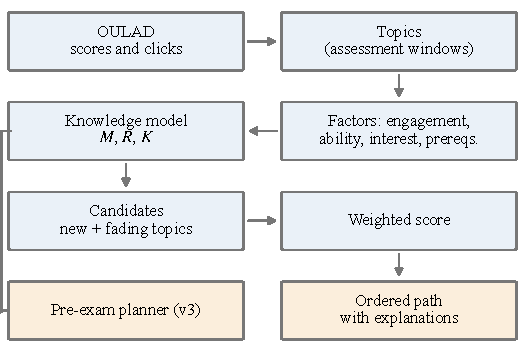
\includegraphics[width=\columnwidth]{figures/pipeline.pdf}
\caption{System pipeline.}
\label{fig:pipeline}
\end{figure}

\subsection{Factors}
For student $s$, topic $k$ and time $t$ the system computes windowed clicks and active days, ability (the shrunk pass rate over topics already assessed), successes and failures on prerequisites, and topic difficulty. The prerequisite graph is the course order. Edges derived from data were considered, but none met the support rule at the planned pass mark. Factors were intended to use only events before $t$. Section~\ref{sec:audit} explains where this failed.

\subsection{Forgetting-Aware PFA (v1, v2)}
For an assessed topic $j$, mastery $M_{s,j}$ is the normalised score and
\begin{align}
R_{s,j}(t) &= 2^{-\Delta_{s,j}(t)/h_{s,j}}, & K_{s,j}(t) &= M_{s,j}R_{s,j}(t),\\
\log_2 h_{s,j} &= \phi_0+\phi_c c_{s,j}+\phi_d d_{s,j}+\phi_I I_{s,j}. \hspace{-8em}
\end{align}
$\Delta$ is the time since submission, or since a later day with at least 3 clicks on the topic's own resources. $c$ and $d$ are clicks and active days, and $h$ is bounded between 1 and 365 days. With $\bar K$ the mean knowledge of the prerequisites,
\begin{equation}
\begin{split}
\operatorname{logit}P(y_{s,k}=1)={}&\beta_k+\theta_a a_s+\theta_K\bar K+\theta_c c_{s,k}\\
&+\theta_I I_{s,k}+\theta_{Ic}I_{s,k}c_{s,k}.
\end{split}
\end{equation}
The variants are no forgetting ($R=1$), fixed exponential decay (time constant \FixedS{} days, chosen on validation), learned half-life, and learned half-life with the interest terms. They are compared with majority, topic difficulty, PFA and DAS3H-style windows, and with DKT as an optional baseline.

\subsection{Interest Proxy}
Interest is proxied by three log click signals: optional resource types, clicks before a topic opens, and clicks after its assessment. Their sum becomes a share of the student's own activity, is standardised against the training cohort, centred within the student and squashed to a value between zero and one. Its correlation with total activity is low ($r=\InterestActivityR$), and its split-half correlation is moderate ($r=\InterestSplitHalf$). It is a behavioural proxy and not measured interest.

\subsection{v3 Memory Model}
v3 changes three things. First, home pages, and forums, subpages and glossaries with evenly spread use (normalised weekly entropy at least 0.80), are navigation and never count as practice. They account for \NavLow{} to \NavHigh{} of clicks by module. Second, the practice on each content resource is attributed to topics. Resources with spread-out use (entropy above 0.4), final-window resources and exam-preparation resources are shared over the topics assessed so far and the current one. Third, retention uses the whole history of doses $x_i$ at times $t_i$:
\begin{align}
m_{s,j}(t) &= \ln\textstyle\sum_{t_i<t} x_i\,(t-t_i+1)^{-d_i},\\
d_i &= c\,e^{m_{s,j}(t_i)}+a,\\
\operatorname{logit}K_{s,j}(t) &= b_0+b_M\operatorname{logit}M_{s,j}+b_m z(m_{s,j}(t)).
\end{align}
Validation selected $a=\DecayA$, $c=\DecayC$ and a submission dose of \DoseSub. Because this $K$ is not on the scale of a score, the preregistered recommender and planner use $MR$, with $R$ the ratio of $K$ now to $K$ just after submission, clipped at one.

\subsection{Candidates, Score and Path}
New topics must be within 2 topics of the current one and have ready prerequisites. Revision topics are those with low $K$. v1 used absolute thresholds, which validation effectively switched off. v2 and v3 flag the lowest 50\% of each student's assessed topics. Candidates are ranked by
\begin{equation}
S=\alpha G+\beta Q+\gamma F+\delta D+\varepsilon I+\zeta\,\mathrm{Pop},
\end{equation}
where $G=1-M$ is the gap, $Q$ the lowest prerequisite $K$, $F=M-K$ the forgetting, $D=1-|K-p^*|/\max(p^*,1-p^*)$ the fit to a target success rate, and Pop (added in v2) the use of the topic by earlier cohorts at the same point. Weights are tuned on validation. A path has up to 5 items, at most 3 of them revisions, with prerequisites first. The largest weighted term supplies each explanation (Fig.~\ref{fig:demo}). In the v3 planner, each of the last 4 weeks before the exam lists the 3 topics with the largest $M-K$ predicted for the exam day.

\begin{figure}[!t]
\centering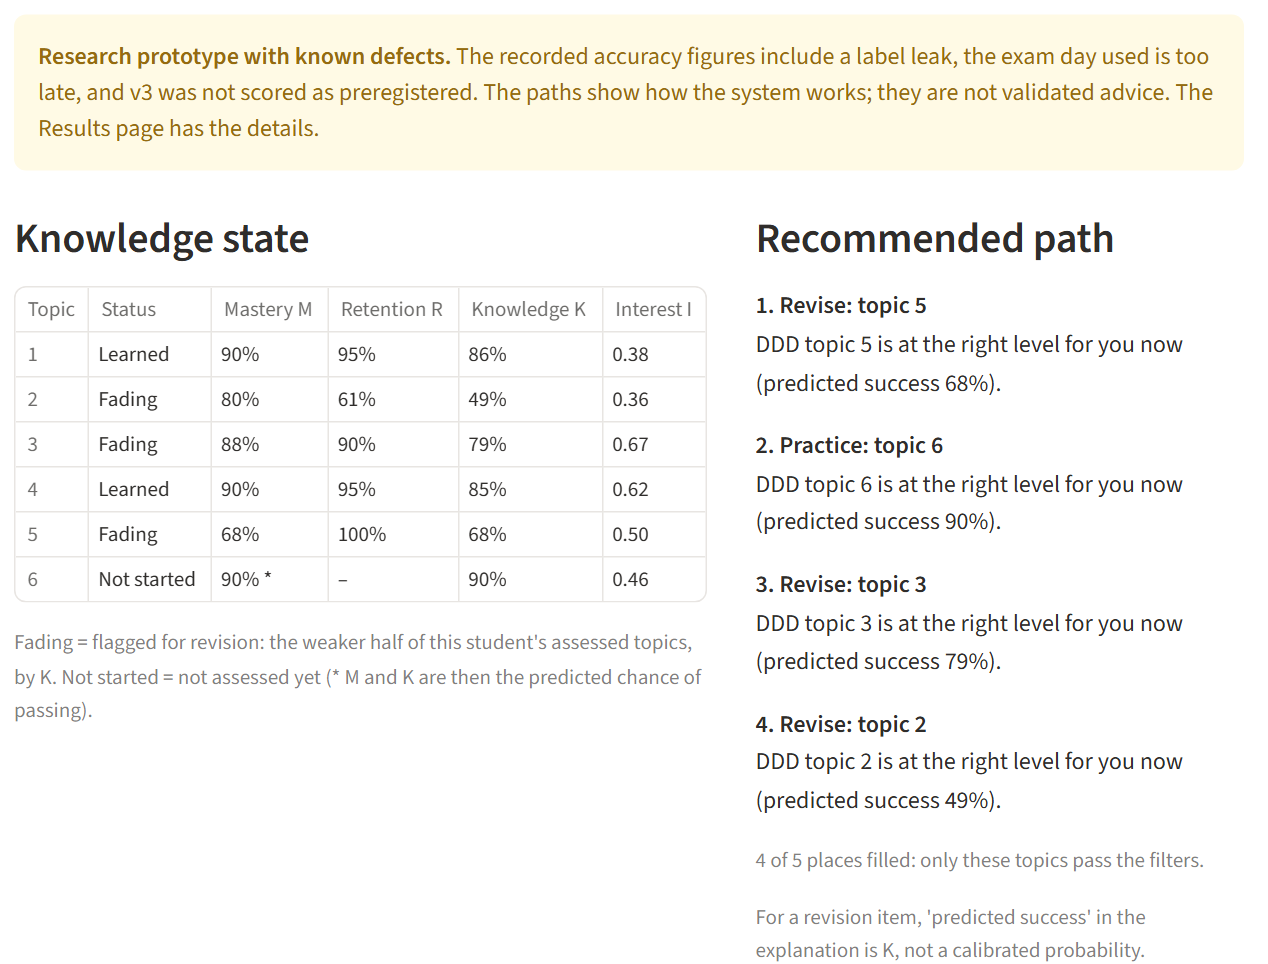
\includegraphics[width=\columnwidth]{figures/demo_crop.png}
\caption{Demonstration, student view: knowledge state and explained path. Paths follow the frozen configuration and illustrate the mechanism. They are not validated advice.}
\label{fig:demo}
\end{figure}

\section{Experimental Protocol}
\subsection{Three Stages}
\emph{v1, planned.} The methodology was fixed in advance. Settings were tuned on 2014B, with logged deviations such as a wider threshold grid, and reported on 2014J, with ablations from random (A0) and popularity (A1) through mastery (A2), prerequisites (A3), fixed forgetting (A4), learned forgetting (A5), interest (A6) and data-derived prerequisites (A7).

\emph{v2, post-hoc.} After the v1 test results were seen, we diagnosed the exam check, made the filters relative, added popularity as a score term (A8 is A5 with it, A9 is A6 with it) and introduced the holdout. Choices were made on validation. v2 results on DDD/FFF 2014J are exploratory.

\emph{v3, post-hoc and preregistered.} The memory model was designed on validation. Variant, settings, comparisons and three criteria were committed before v3 was scored elsewhere. The criteria were: (a) holdout within-course AUC no worse than v2 by more than 0.002, (b) a CCC exam gap above v2's $-0.096$ with the interval of the improvement above 0, and (c) holdout NDCG@5 of A5 at least that of v2. (a) and (c) are primary. (b) and everything on DDD/FFF 2014J are exploratory. The holdout was not fresh for v3, because its v2 results had been seen.

\subsection{Measures}
Prediction is measured by AUC, log-loss and Brier score. For ranking, Rel-A marks topics with at least 10 clicks in the following window among students who then passed, and Rel-B marks the current topic and up to 2 before it among students who then failed. Combined relevance pools both. The exam check compares the Spearman correlation with the exam score of mean $K$ and of mean $M$. A positive gap would favour decayed knowledge. Intervals are 95\% bootstrap intervals over students (1{,}000 resamples, and 200 for coefficients). Ranking comparisons use paired Wilcoxon tests with Holm correction.

\subsection{Audit of the Evaluation}\label{sec:audit}
While preparing this report we re-read the code and checked it against the stored data without refitting. We found four defects.

\emph{D1, label leakage.} A row for topic $k$ is predicted at its due date, and ability averages all results submitted earlier. An early submitter's own label is therefore in the feature. This holds for \LeakMain{} of DDD/FFF test rows and for \LeakLow{} to \LeakHigh{} on the holdout (Table~\ref{tab:leak}). On topic 1, where there is no history, ability alone reaches an AUC of \LeakAucDDD{} in DDD and \LeakAucFFF{} in FFF. In CCC, where no topic 1 row is affected, it reaches \LeakAucCCC. Post-submission clicks enter other features of the same rows. Every predictive metric, and every choice tuned on one, is contaminated. The original leakage tests passed because they altered only events after the prediction time.

\emph{D2, exam day.} The exam was placed on the last day of the presentation. The median recorded sitting is \LateMin{} to \LateMax{} days earlier (Table~\ref{tab:examday}), so ``knowledge at the exam'' includes later activity. In CCC 2014J, \LateWeeksCCC{} of the planner's 4 weeks fall after the median exam.

\emph{D3, departure from the preregistration.} The preregistration and frozen configuration specify $MR$ for the recommender and planner. The scoring script used raw $K$ outside validation. The stored plans and the A5 ranking scores are reproduced exactly with raw $K$, and the preregistered scale gives plan values that differ by up to \ScaleGap. The correctly configured results were not computed and are unknown.

\emph{D4, look-ahead in cohort features.} Topic maps, navigation classes and attribution weights use the scored cohort's own clicks over the whole course. Contrary to our log, the shared rule also reads the revision period, which changes the class of \SitesMain{} DDD/FFF and \SitesCCC{} CCC resources.

Results below are unchanged. They describe what was recorded, not what is established.

% generated by report/make_tables.py - do not edit
% sources: report/audit/first_topic_ability_auc.csv, report/audit/label_in_ability.csv
\begin{table}[!t]
\centering
\caption{D1: label inside the ability feature, 2014J test rows. Read-only audit (D1)}
\label{tab:leak}
\scriptsize
\setlength{\tabcolsep}{3pt}
\begin{tabular}{@{}llll@{}}
\toprule
Module & All rows & Topic 1 & AUC, topic 1 \\
\midrule
DDD & 52\% & 66\% & 0.875 \\
FFF & 61\% & 70\% & 0.920 \\
AAA & 35\% & 39\% & 0.700 \\
BBB & 68\% & 84\% & 0.988 \\
CCC & 18\% & 0\% & 0.510 \\
EEE & 57\% & 65\% & 0.865 \\
GGG & 70\% & 78\% & 0.928 \\
\bottomrule
\end{tabular}
\par\vspace{2pt}\parbox{\linewidth}{\scriptsize Read-only count on stored data. Topic 1 has no history, so a clean feature scores 0.5.}
\end{table}


\section{Results}
\subsection{v1: Planned Analysis}
Table~\ref{tab:pred-v1} gives the recorded prediction metrics. The learned half-life reached an AUC of \AucLearned, against \AucNone{} without forgetting (paired difference \AucGain, interval \AucGainLo{} to \AucGainHi). The model with only topic and ability already reached \AucTopicOne. D1 makes all of these invalid as estimates of performance, and the comparison with DKT, which lacks the ability feature, is not like for like (Table~\ref{tab:dkt}).

In ranking (Table~\ref{tab:rank-v1}), A5 scored \RankFive{} and A3 \RankThree{} on combined relevance, with most of the difference on Rel-B (\RankFiveB{} against \RankThreeB). That A3 had been tuned to rank by readiness alone, so it was a weak reference. Popularity scored \RankPop. Random scored \RankRandom, more than mastery alone (\RankMastery), which shows how forgiving the measure is with so few topics. The A5--A3 difference kept its sign with a pass mark of 70 (\SensSeventy) and with non-submission counted as failure (\SensNonsub). It reversed with data-derived prerequisites at the higher pass mark (\SensData). These rankings depend on coefficients and settings fitted under D1.

The exam check went against the forgetting hypothesis: the gap for the learned decay was \ExamGap{} on DDD (Table~\ref{tab:exam}). This check is subject to D2.

% generated by report/make_tables.py - do not edit
% sources: results/tables/ranking_metrics_test.csv
\begin{table}[!t]
\centering
\caption{v1 ablation, DDD/FFF 2014J test, NDCG@5. Planned analysis (D1)}
\label{tab:rank-v1}
\scriptsize
\setlength{\tabcolsep}{3pt}
\begin{tabular}{@{}llll@{}}
\toprule
Configuration & Combined [95\% CI] & Rel-A & Rel-B \\
\midrule
A0 Random & 0.739 [0.734, 0.744] & 0.737 & 0.726 \\
A1 Popularity & 0.946 [0.944, 0.949] & 0.952 & 0.824 \\
A2 Mastery & 0.653 [0.648, 0.658] & 0.648 & 0.698 \\
A3 + prerequisites & 0.828 [0.823, 0.833] & 0.840 & 0.553 \\
A4 + fixed decay & 0.843 [0.839, 0.848] & 0.841 & 0.824 \\
A5 + learned decay & 0.840 [0.835, 0.844] & 0.838 & 0.805 \\
A6 + interest & 0.837 [0.833, 0.842] & 0.836 & 0.802 \\
A7 + data edges & 0.837 [0.833, 0.842] & 0.836 & 0.802 \\
\bottomrule
\end{tabular}
\par\vspace{2pt}\parbox{\linewidth}{\scriptsize Indirectly affected by the leak (D1) through fitted coefficients and tuned settings; A0 and A1 fit no model.}
\end{table}


\subsection{v2: Post-Hoc Fixes and Holdout}
The diagnosis on validation (Fig.~\ref{fig:diag}) found that middle topics are rarely reopened. Their median $\Delta$ at the assumed exam day ranges from \DeltaFive{} to \DeltaTwo{} days, and only \ResetFive{} to \ResetThree{} of students reset their clock on them, against \ResetSix{} for the final topic. The clock arithmetic was correct, but this audit did not notice that the exam day itself was wrong.

On the holdout, the recorded AUC difference between learned decay and no forgetting was \HoldGain{} (interval \HoldGainLo{} to \HoldGainHi), and DAS3H was ahead of the learned model by \HoldDasGap{} (Table~\ref{tab:pred-v2}). In ranking (Fig.~\ref{fig:ndcg}, Table~\ref{tab:rank-holdout}), A5 minus A3 was \HoldForget{} on combined relevance and \HoldForgetB{} on Rel-B. A9 minus A8, the interest contrast, was \HoldInterest. Popularity scored \HoldPop, and A8 trailed it by \HoldPopGap. Popularity uses only earlier cohorts and fits no model, so it is the result least affected by D1. In the exploratory run on DDD/FFF 2014J, A5 minus A3 was \PostForget.

\begin{figure}[!t]
\centering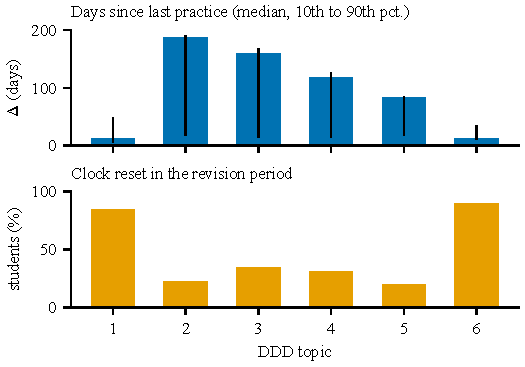
\includegraphics[width=\columnwidth]{figures/exam_diagnosis.pdf}
\caption{Exam diagnosis, DDD 2014B (post-hoc, validation). ``At the exam'' means the last day of the presentation, which is after the real exam (D2).}
\label{fig:diag}
\end{figure}

\begin{figure}[!t]
\centering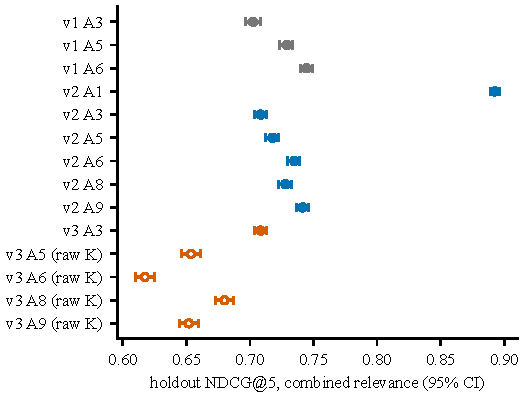
\includegraphics[width=\columnwidth]{figures/ndcg_holdout.pdf}
\caption{Holdout ranking (post-hoc, v3 preregistered). Hollow points were scored with raw $K$ and not as preregistered (D3). Model-based configurations are indirectly affected by D1.}
\label{fig:ndcg}
\end{figure}

% generated by report/make_tables.py - do not edit
% sources: results/v2/holdout/ranking_metrics_holdout.csv, results/v3/holdout/recommender_holdout.csv
\begin{table}[!t]
\centering
\caption{Holdout NDCG@5 across stages. v1 configurations and v2: post-hoc. v3: post-hoc, preregistered (D1, D3)}
\label{tab:rank-holdout}
\scriptsize
\setlength{\tabcolsep}{3pt}
\begin{tabular}{@{}llll@{}}
\toprule
Configuration & Combined [95\% CI] & Rel-A & Rel-B \\
\midrule
v1 A3 & 0.702 [0.696, 0.708] & 0.700 & 0.635 \\
v1 A5 & 0.729 [0.724, 0.733] & 0.722 & 0.768 \\
v1 A6 & 0.745 [0.740, 0.749] & 0.738 & 0.775 \\
v2 A1 & 0.893 [0.889, 0.896] & 0.893 & 0.879 \\
v2 A3 & 0.708 [0.703, 0.713] & 0.704 & 0.720 \\
v2 A5 & 0.718 [0.712, 0.723] & 0.714 & 0.717 \\
v2 A6 & 0.735 [0.730, 0.739] & 0.731 & 0.725 \\
v2 A8 & 0.728 [0.723, 0.733] & 0.724 & 0.731 \\
v2 A9 & 0.742 [0.737, 0.746] & 0.738 & 0.734 \\
v3 A3 & 0.708 [0.703, 0.713] & 0.704 & 0.720 \\
v3 A5 (raw K) & 0.654 [0.646, 0.661] & 0.656 & 0.486 \\
v3 A6 (raw K) & 0.617 [0.610, 0.625] & 0.619 & 0.470 \\
v3 A8 (raw K) & 0.680 [0.673, 0.687] & 0.680 & 0.558 \\
v3 A9 (raw K) & 0.652 [0.645, 0.659] & 0.651 & 0.548 \\
\bottomrule
\end{tabular}
\par\vspace{2pt}\parbox{\linewidth}{\scriptsize v3 rows were scored with raw K instead of the preregistered $K=MR$ (D3). Indirectly affected by the leak (D1) through fitted coefficients and tuned settings; A0 and A1 fit no model.}
\end{table}


\subsection{v3: Preregistered Memory Revision}
With shared attribution, \VisSharedLow{} to \VisSharedHigh{} of DDD validation exam-takers have a revision dose on topics 2 to 5, against \VisDirectLow{} to \VisDirectHigh{} with direct attribution of content. Part of this rise is mechanical, because one click on a shared resource is credited to several topics. Fig.~\ref{fig:curve} shows the two memory models for one student. On validation no variant reached a non-negative exam gap, so the fallback rule selected the spacing-sensitive activation model (Table~\ref{tab:variants}). With $MR$, A5 scored \ScaleScore{} on validation, against \ScaleRaw{} with raw $K$ and \ValVTwo{} for v2.

Table~\ref{tab:criteria} and Fig.~\ref{fig:criteria} give the criteria as recorded.

\emph{(a) was met.} Holdout AUC was \CritAThree{} for v3 and \CritATwo{} for v2 (difference \CritADiff, interval \CritALo{} to \CritAHi). Both models contain D1.

\emph{(b) was met (exploratory).} The CCC gap moved from \CritBTwo{} to \CritBThree{} (improvement \CritBDiff, interval \CritBLo{} to \CritBHi). It is still negative, so decayed knowledge remained a worse exam predictor than mastery. The criterion would also be met by no forgetting at all, whose gap is zero by definition, and the exam day is wrong.

\emph{(c) was not met.} v3 A5 scored \CritCThree{} against \CritCTwo{} for v2. This is a failure of what was run, which was not the preregistered configuration (D3). It shows neither that the preregistered recommender fails nor that it would have passed.

\begin{figure}[!t]
\centering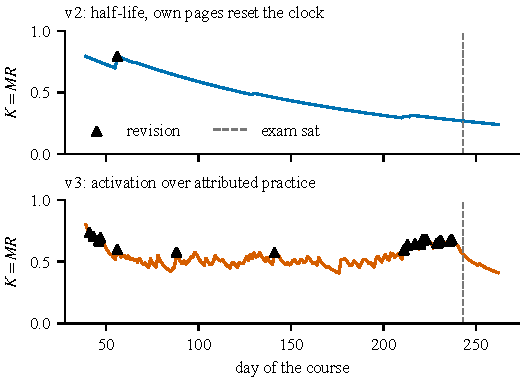
\includegraphics[width=\columnwidth]{figures/forgetting.pdf}
\caption{Example: topic 2 of the demonstration's default DDD student, chosen by a fixed rule. Post-hoc illustration on 2014J. Both curves continue past the day the exam was sat.}
\label{fig:curve}
\end{figure}

\begin{figure}[!t]
\centering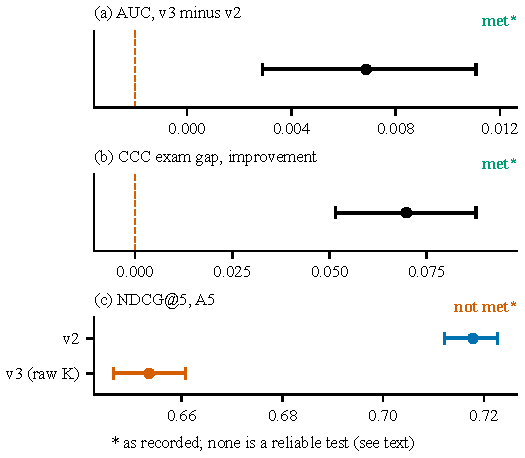
\includegraphics[width=\columnwidth]{figures/criteria.pdf}
\caption{Preregistered v3 criteria as recorded: (a), (c) primary, (b) exploratory. Dashed lines are thresholds. (a) contains D1, (b) D2, and (c) was not scored as preregistered (D3).}
\label{fig:criteria}
\end{figure}

% generated by report/make_tables.py - do not edit
% sources: results/v3/holdout/exam_check_CCC.csv, results/v3/holdout/model_metrics_holdout.csv, results/v3/holdout/recommender_holdout.csv, results/v3/holdout/recommender_wilcoxon_holdout.csv
\begin{table*}[!t]
\centering
\caption{Preregistered v3 criteria, as recorded. v3, post-hoc and preregistered. (a) and (c) primary, (b) exploratory. Statuses as recorded (D1, D2, D3)}
\label{tab:criteria}
\scriptsize
\setlength{\tabcolsep}{3pt}
\begin{tabular}{@{}>{\raggedright\arraybackslash}p{3.5cm}>{\raggedright\arraybackslash}p{2.0cm}>{\raggedright\arraybackslash}p{2.0cm}>{\raggedright\arraybackslash}p{2.7cm}>{\raggedright\arraybackslash}p{1.3cm}>{\raggedright\arraybackslash}p{1.3cm}>{\raggedright\arraybackslash}p{2.9cm}@{}}
\toprule
Criterion & v3 & v2 & v3 minus v2 & Recorded & Evidence & Can it be relied on? \\
\midrule
(a) Holdout within-course AUC at most 0.002 below v2 & 0.848 [0.838, 0.859] & 0.841 [0.831, 0.851] & $+$0.007 [$+$0.003, $+$0.011] & MET & primary & No: both models contain the label leak (D1). \\
(b) CCC exam gap above v2's, CI of the improvement above 0 & $-$0.026 & $-$0.096 & $+$0.070 [$+$0.052, $+$0.088] & MET & exploratory & No: wrong exam day (D2), and a model with no forgetting (gap = 0) would also pass. \\
(c) Holdout NDCG@5 of v3 A5 at least v2 A5 & 0.654 [0.646, 0.661] & 0.718 [0.712, 0.723] & $-$0.064 & NOT MET & primary & No: scored with raw K, not the preregistered configuration (D3). \\
\bottomrule
\end{tabular}
\par\vspace{2pt}\parbox{\linewidth}{\scriptsize The recorded statuses are unchanged; none is a reliable test.}
\end{table*}

% generated by report/make_tables.py - do not edit
% sources: results/tables/exam_retention_check.csv, results/v2/holdout/exam_retention_check_holdout.csv, results/v3/holdout/exam_check_CCC.csv, results/v3/planner/exam_check_val.csv, results/v3/posthoc_2014J/exam_check_DDD_2014J.csv
\begin{table}[!t]
\centering
\caption{Exam check: rank correlation of K minus that of M. v1 planned. v2 and v3 post-hoc and exploratory (D1, D2)}
\label{tab:exam}
\footnotesize
\setlength{\tabcolsep}{3pt}
\begin{tabular}{@{}>{\raggedright\arraybackslash}p{2.3cm}ll@{}}
\toprule
Model and set & Gap [95\% CI] & Change from v2 \\
\midrule
v1 fixed, DDD 2014J (planned) & $-$0.152 [$-$0.192, $-$0.104] & -- \\
v1 learned, DDD 2014J (planned) & $-$0.088 [$-$0.123, $-$0.050] & -- \\
v2 fixed, CCC (exploratory) & $-$0.298 [$-$0.337, $-$0.262] & -- \\
v2 learned, CCC (exploratory) & $-$0.096 [$-$0.113, $-$0.078] & -- \\
v3, DDD 2014B (validation) & $-$0.008 & $+$0.089 [$+$0.048, $+$0.134] \\
v3, CCC (exploratory) & $-$0.026 & $+$0.070 [$+$0.052, $+$0.088] \\
v3, DDD 2014J (exploratory) & $-$0.012 & $+$0.076 [$+$0.042, $+$0.110] \\
\bottomrule
\end{tabular}
\par\vspace{2pt}\parbox{\linewidth}{\scriptsize Unreliable: 'exam day' is the last day of the presentation, after the real exam (D2); coefficients carry D1.}
\end{table}


\subsection{Interest and Planner}
In v1 two interest coefficients had intervals above zero and the interaction did not (Table~\ref{tab:interest}). The interest model did not predict better, and the tuned weight of interest in the score was zero in every configuration. The ranking contrast was negative in v1, positive on the holdout in v2 and negative in v3 as scored. We do not conclude that interest helps.

The planner produces readable weekly plans, but there is no evidence that it helps. The association between revising flagged topics and the exam score was negative on validation and CCC and inconclusive on DDD 2014J (Table~\ref{tab:planner}). It is observational, confounded by who chooses to revise what, and affected by D2 and, outside validation, D3.

\section{Discussion}
\emph{Does forgetting help?} This evaluation cannot say. The prediction differences are small next to a leak of the label itself, and they cannot be corrected by inspection. The ranking gains change with the reference configuration and the stage. No exam check found decayed knowledge ahead of plain mastery, but all of them use the wrong day.

\emph{What did v3 achieve?} It implemented a plausible remedy for invisible revision and a richer memory model. Its two criteria recorded as met are weaker than they look. In CCC the fitted weight on activation is \BmActivation, against \BmMastery{} on the logit of mastery, so $K$ there is close to a function of $M$ alone. A gap that shrinks towards zero can mean that the model forgets less, not that it models forgetting better. Its recommender has not yet been tested as specified.

\emph{Learned or fixed decay?} The learned half-life was less negative than the fixed decay on both recorded exam checks, while fixed decay ranked slightly better in v1. Neither observation is reliable enough to choose between them.

\emph{What does ranking measure here?} Rel-A rewards what cohorts usually do next, which is what popularity predicts. Rel-B is a fixed function of the current topic, so a rule that always lists that topic and the two before it would be perfect on it without personalisation. The baselines also rank an unfiltered set, while the proposed configurations return shorter filtered lists. The frozen v3 A5 puts all weight on $D$. For $K$ below $p^*=0.9$ this term grows with $K$, so the best-retained revision topic comes first, which is the opposite of the intended behaviour.

\emph{What did the process teach us?} Preregistration fixed the criteria but did not check that the code implemented them. Reproduction from a clean clone matched every table and reproduced every bug. Tests that perturb the future cannot find a label that arrives early. A one-feature model on a row with no history, a plot of activity around the assumed exam day, and an assertion that the scoring configuration equals the frozen one would each have exposed a defect early.

\section{Limitations and Future Work}
Beyond D1 to D4, topics are assessment windows and not concepts, prerequisites are course order, and the first topic absorbs course-wide resources. Passing is near its ceiling, and excluding non-submission removes much of what failure means in this dataset. Results are treated as known on the submission day, although marking takes time. Some students appear in more than one presentation or module. Offline relevance is not learning, the simulated gains reported in the repository are model-based, and interest cannot be separated from motivation or deadlines.

The first task is a corrected evaluation, registered as new work:
\begin{enumerate}
\item compute every feature for topic $k$ strictly before the earlier of its due date and the student's submission, and exclude $k$ from ability;
\item use each student's recorded sitting day for the exam check and planner;
\item derive cohort features from earlier presentations, or only from days before the prediction time;
\item score exactly the frozen configuration, asserted in code, and then repeat selection, tuning and all three stages;
\item compare with trivial baselines, including the fixed rule for Rel-B and no forgetting for the exam check.
\end{enumerate}
Since all the test sets have been seen, a confirmatory claim would need new data. Whether recommended revision improves learning needs a controlled study.

\section{Conclusion}
We built a complete, interpretable learning-path system with mastery, forgetting, prerequisites, interest, explanations, a revision planner and a working demonstration. Its evaluation does not establish the midterm hypothesis. As recorded, the preregistered revision met its prediction and exploratory exam criteria and failed its ranking criterion. The audit shows that the first two are not reliable and that the third did not test the registered system. Popularity remained the strongest recommender under our offline measures, and no benefit of interest or of the planner was demonstrated. The next step is the corrected evaluation described above.

\appendices
\section{Recorded Results in Full}
All values below are generated from the frozen result files. The caption of each table gives its status.

% generated by report/make_tables.py - do not edit
% sources: results/tables/model_metrics_test.csv
\begin{table}[!t]
\centering
\caption{v1 knowledge models, DDD/FFF 2014J test. Planned analysis (D1)}
\label{tab:pred-v1}
\scriptsize
\setlength{\tabcolsep}{3pt}
\begin{tabular}{@{}llll@{}}
\toprule
Model & AUC [95\% CI] & Log-loss & Brier \\
\midrule
Majority & 0.500 & 0.186 & 0.043 \\
Topic difficulty & 0.848 [0.833, 0.863] & 0.138 & 0.034 \\
PFA & 0.890 [0.876, 0.903] & 0.131 & 0.033 \\
No forgetting & 0.900 [0.888, 0.912] & 0.129 & 0.033 \\
Fixed decay & 0.900 [0.888, 0.911] & 0.129 & 0.034 \\
Learned half-life & 0.902 [0.890, 0.914] & 0.128 & 0.033 \\
Half-life + interest & 0.900 [0.888, 0.912] & 0.128 & 0.033 \\
DAS3H windows & 0.889 [0.875, 0.902] & 0.133 & 0.033 \\
\bottomrule
\end{tabular}
\par\vspace{2pt}\parbox{\linewidth}{\scriptsize Invalid as performance: the label leaks into the ability feature (D1).}
\end{table}

% generated by report/make_tables.py - do not edit
% sources: results/v2/holdout/model_metrics_holdout.csv
\begin{table}[!t]
\centering
\caption{v2 knowledge models, five holdout modules (pooled). Post-hoc (D1)}
\label{tab:pred-v2}
\footnotesize
\setlength{\tabcolsep}{3pt}
\begin{tabular}{@{}lll@{}}
\toprule
Model & AUC [95\% CI] & Log-loss \\
\midrule
Topic difficulty & 0.821 [0.809, 0.833] & 0.197 \\
PFA & 0.854 [0.843, 0.865] & 0.184 \\
No forgetting & 0.848 [0.838, 0.857] & 0.202 \\
Fixed decay & 0.847 [0.837, 0.857] & 0.203 \\
Learned half-life & 0.847 [0.837, 0.857] & 0.203 \\
Half-life + interest & 0.847 [0.837, 0.857] & 0.201 \\
DAS3H windows & 0.858 [0.846, 0.869] & 0.179 \\
\bottomrule
\end{tabular}
\par\vspace{2pt}\parbox{\linewidth}{\scriptsize Invalid as performance: the label leaks into the ability feature (D1).}
\end{table}

% generated by report/make_tables.py - do not edit
% sources: results/v3/holdout/model_metrics_holdout.csv, results/v3/posthoc_2014J/model_metrics_2014J.csv
\begin{table}[!t]
\centering
\caption{v3 against v2, within-course AUC. Post-hoc, preregistered (D1)}
\label{tab:pred-v3}
\scriptsize
\setlength{\tabcolsep}{3pt}
\begin{tabular}{@{}>{\raggedright\arraybackslash}p{2.2cm}lll@{}}
\toprule
Set & v2 & v3 & Difference [95\% CI] \\
\midrule
Holdout (primary) & 0.841 & 0.848 & $+$0.007 [$+$0.003, $+$0.011] \\
DDD/FFF 2014J (exploratory) & 0.906 & 0.910 & $+$0.005 [0.000, $+$0.009] \\
\bottomrule
\end{tabular}
\par\vspace{2pt}\parbox{\linewidth}{\scriptsize Invalid as performance: the label leaks into the ability feature (D1).}
\end{table}

% generated by report/make_tables.py - do not edit
% sources: results/tables/dkt_comparison.csv
\begin{table}[!t]
\centering
\caption{Optional DKT baseline, test rows with history. Planned optional baseline (D1)}
\label{tab:dkt}
\footnotesize
\setlength{\tabcolsep}{3pt}
\begin{tabular}{@{}ll@{}}
\toprule
Model & AUC [95\% CI] \\
\midrule
DKT (no ability feature) & 0.783 [0.764, 0.801] \\
PFA & 0.882 [0.868, 0.895] \\
Learned half-life & 0.898 [0.886, 0.910] \\
\bottomrule
\end{tabular}
\par\vspace{2pt}\parbox{\linewidth}{\scriptsize Not like for like: DKT lacks the leaking feature that the other models have (D1).}
\end{table}

% generated by report/make_tables.py - do not edit
% sources: results/v2/posthoc_2014J/ranking_metrics.csv, results/v3/posthoc_2014J/recommender_2014J.csv
\begin{table}[!t]
\centering
\caption{v2 and v3 on DDD/FFF 2014J, NDCG@5 (exploratory). Post-hoc, exploratory (D1, D3)}
\label{tab:rank-2014j}
\scriptsize
\setlength{\tabcolsep}{3pt}
\begin{tabular}{@{}llll@{}}
\toprule
Configuration & Combined [95\% CI] & Rel-A & Rel-B \\
\midrule
v2 A1 & 0.946 [0.944, 0.949] & 0.952 & 0.824 \\
v2 A3 & 0.784 [0.780, 0.789] & 0.783 & 0.756 \\
v2 A5 & 0.784 [0.779, 0.789] & 0.784 & 0.723 \\
v2 A6 & 0.786 [0.782, 0.791] & 0.786 & 0.718 \\
v2 A8 & 0.794 [0.790, 0.799] & 0.795 & 0.723 \\
v2 A9 & 0.797 [0.792, 0.802] & 0.798 & 0.721 \\
v3 A5 (raw K) & 0.730 [0.724, 0.738] & 0.735 & 0.529 \\
v3 A6 (raw K) & 0.723 [0.716, 0.730] & 0.729 & 0.507 \\
v3 A8 (raw K) & 0.774 [0.768, 0.781] & 0.781 & 0.557 \\
v3 A9 (raw K) & 0.767 [0.761, 0.774] & 0.775 & 0.537 \\
\bottomrule
\end{tabular}
\par\vspace{2pt}\parbox{\linewidth}{\scriptsize v3 rows were scored with raw K instead of the preregistered $K=MR$ (D3). Indirectly affected by the leak (D1) through fitted coefficients and tuned settings; A0 and A1 fit no model.}
\end{table}

% generated by report/make_tables.py - do not edit
% sources: results/tables/wilcoxon_holm.csv, results/v2/holdout/wilcoxon_holm_holdout.csv, results/v3/holdout/recommender_wilcoxon_holdout.csv
\begin{table}[!t]
\centering
\caption{Paired Wilcoxon tests on NDCG@5, Holm-corrected. v1 planned. v2 and v3 post-hoc (D1, D3)}
\label{tab:tests}
\footnotesize
\setlength{\tabcolsep}{3pt}
\begin{tabular}{@{}lrr@{}}
\toprule
Comparison & Difference & Holm p \\
\midrule
v1 test: A5 vs A3 & $+$0.012 & $<$0.0001 \\
v1 test: A5 vs A4 & $-$0.004 & $<$0.0001 \\
v1 test: A6 vs A5 & $-$0.003 & $<$0.0001 \\
v2 holdout: A5 vs A3 & $+$0.009 & $<$0.0001 \\
v2 holdout: A8 vs A1 & $-$0.165 & $<$0.0001 \\
v2 holdout: A9 vs A8 & $+$0.014 & $<$0.0001 \\
v3 holdout: A5 vs v2 A5 & $-$0.064 & $<$0.0001 \\
v3 holdout: A5 vs A3 & $-$0.055 & $<$0.0001 \\
v3 holdout: A9 vs A8 & $-$0.028 & $<$0.0001 \\
\bottomrule
\end{tabular}
\par\vspace{2pt}\parbox{\linewidth}{\scriptsize v3 rows were scored with raw K instead of the preregistered $K=MR$ (D3). Indirectly affected by the leak (D1) through fitted coefficients and tuned settings; A0 and A1 fit no model.}
\end{table}

% generated by report/make_tables.py - do not edit
% sources: results/v3/variant_comparison_val.csv
\begin{table}[!t]
\centering
\caption{v3 memory variants on validation. Post-hoc, validation only (D1, D2)}
\label{tab:variants}
\scriptsize
\setlength{\tabcolsep}{3pt}
\begin{tabular}{@{}>{\raggedright\arraybackslash}p{3.7cm}lll@{}}
\toprule
Variant & Log-loss & AUC & Exam gap \\
\midrule
V0 v2 half-life & 0.1613 & 0.898 & $-$0.097 \\
V1 half-life, attributed & 0.1616 & 0.898 & $-$0.041 \\
V2 ACT-R, fixed decay & 0.1578 & 0.903 & $-$0.014 \\
V3 ACT-R, spacing (selected) & 0.1580 & 0.902 & $-$0.008 \\
V4 DAS3H, attributed & 0.1623 & 0.885 & $-$0.168 \\
\bottomrule
\end{tabular}
\par\vspace{2pt}\parbox{\linewidth}{\scriptsize Selection used leaking losses (D1) and the wrong exam day (D2).}
\end{table}

% generated by report/make_tables.py - do not edit
% sources: results/tables/coefficients.csv
\begin{table}[!t]
\centering
\caption{v1 interest coefficients. Planned analysis, training fit (D1)}
\label{tab:interest}
\footnotesize
\setlength{\tabcolsep}{3pt}
\begin{tabular}{@{}ll@{}}
\toprule
Coefficient & Estimate [95\% CI] \\
\midrule
Interest on half-life & $+$0.566 [$+$0.058, $+$0.966] \\
Interest on passing & $+$0.144 [$+$0.059, $+$0.237] \\
Interest x clicks & $+$0.035 [$-$0.013, $+$0.098] \\
\bottomrule
\end{tabular}
\par\vspace{2pt}\parbox{\linewidth}{\scriptsize Fitted with the leak (D1); the interest feature also sees post-submission clicks.}
\end{table}

% generated by report/make_tables.py - do not edit
% sources: results/v3/holdout/observational_check_CCC.csv, results/v3/planner/observational_check_val.csv, results/v3/posthoc_2014J/observational_check_DDD_2014J.csv
\begin{table}[!t]
\centering
\caption{Planner: observational association, not causal. Post-hoc, exploratory (D2, D3)}
\label{tab:planner}
\footnotesize
\setlength{\tabcolsep}{3pt}
\begin{tabular}{@{}>{\raggedright\arraybackslash}p{3.4cm}rl@{}}
\toprule
Set & n & Coefficient [95\% CI] \\
\midrule
DDD 2014B (validation, $MR$) & 472 & $-$21.5 [$-$37.5, $-$7.1] \\
CCC (exploratory, raw K) & 823 & $-$22.5 [$-$28.4, $-$16.6] \\
DDD 2014J (exploratory, raw K) & 865 & 6.5 [$-$7.8, 20.4] \\
\bottomrule
\end{tabular}
\par\vspace{2pt}\parbox{\linewidth}{\scriptsize Not causal. Much of the 'pre-exam' window is after the exam (D2); raw K outside validation (D3).}
\end{table}

% generated by report/make_tables.py - do not edit
% sources: report/audit/exam_day.csv
\begin{table}[!t]
\centering
\caption{D2: exam day used against the day it was sat. Read-only audit (D2)}
\label{tab:examday}
\scriptsize
\setlength{\tabcolsep}{3pt}
\begin{tabular}{@{}llll@{}}
\toprule
Presentation & Day used & Day sat & Weeks late \\
\midrule
DDD 2014B & 241 & 234 & 1 \\
DDD 2014J & 262 & 243 & 2 \\
CCC 2014B & 241 & 230 & 1 \\
CCC 2014J & 269 & 244 & 3 \\
\bottomrule
\end{tabular}
\par\vspace{2pt}\parbox{\linewidth}{\scriptsize Read-only comparison with the recorded sitting day.}
\end{table}


\bibliographystyle{IEEEtran}
\bibliography{references}

\end{document}
